\subsection{Medium BDT Score Sidebands}
\label{sec:MediumBDTScoreSidebands}

We can inspect the full energy spectrum whilst keeping the signal region blind by applying cuts to the BDT scores. The medium BDT score sidebands are constructed by selecting events from the near sidebands with background scores between 0.4 and 0.72 in the case of the 1e0p selection. When applying the 1eNp selection, we only include events that have both $0.1<$ $\pi^0$ score $< 0.67$, and $0.1<$ non-$\pi^0$ score $< 0.70$. 

\begin{figure}[H]
    \centering
    \begin{subfigure}{0.5\linewidth}
        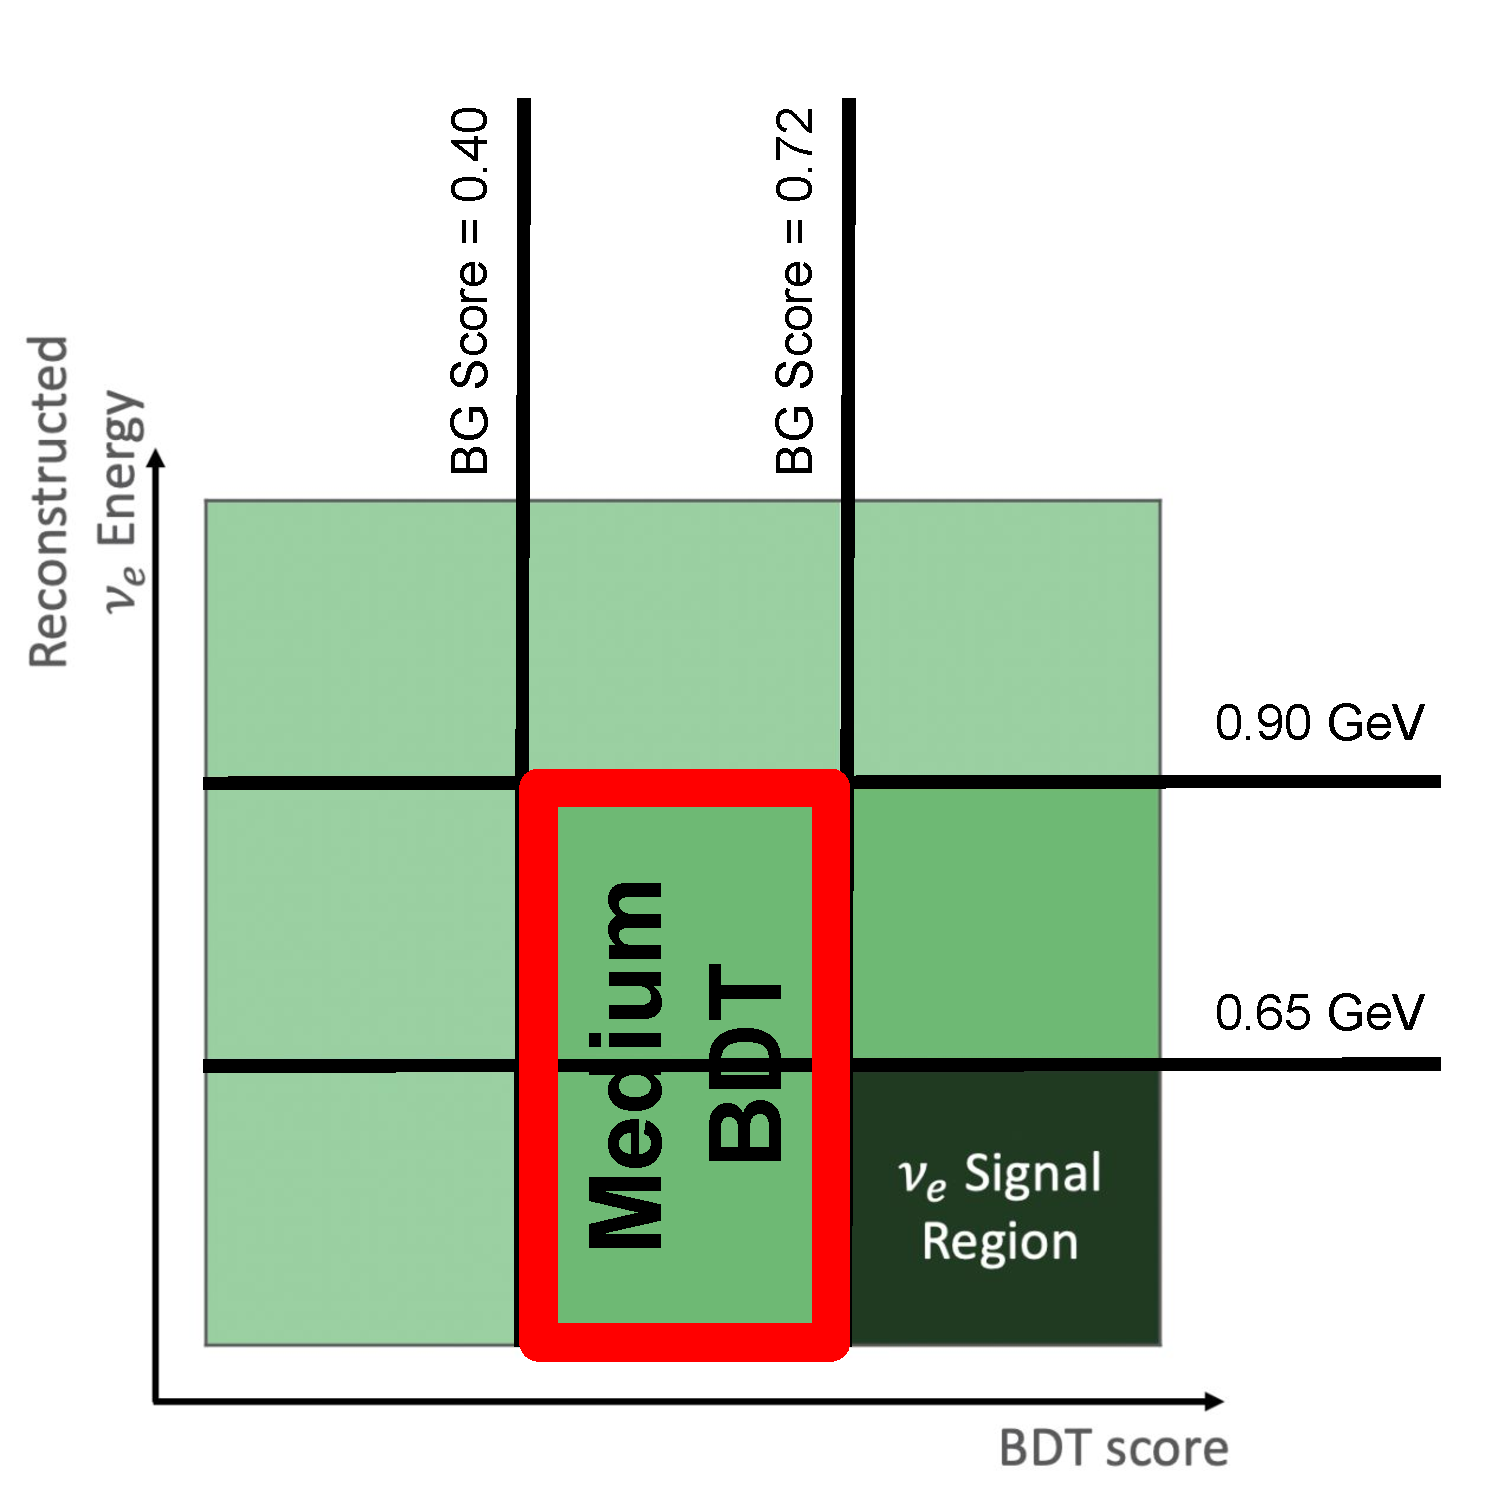
\includegraphics[width=\linewidth]{technote/Sidebands/Figures/NearSideband/ZpMediumBDTSideband.pdf}
        \caption{For the 1e0p selection.}
    \end{subfigure}%
    \begin{subfigure}{0.5\linewidth}
        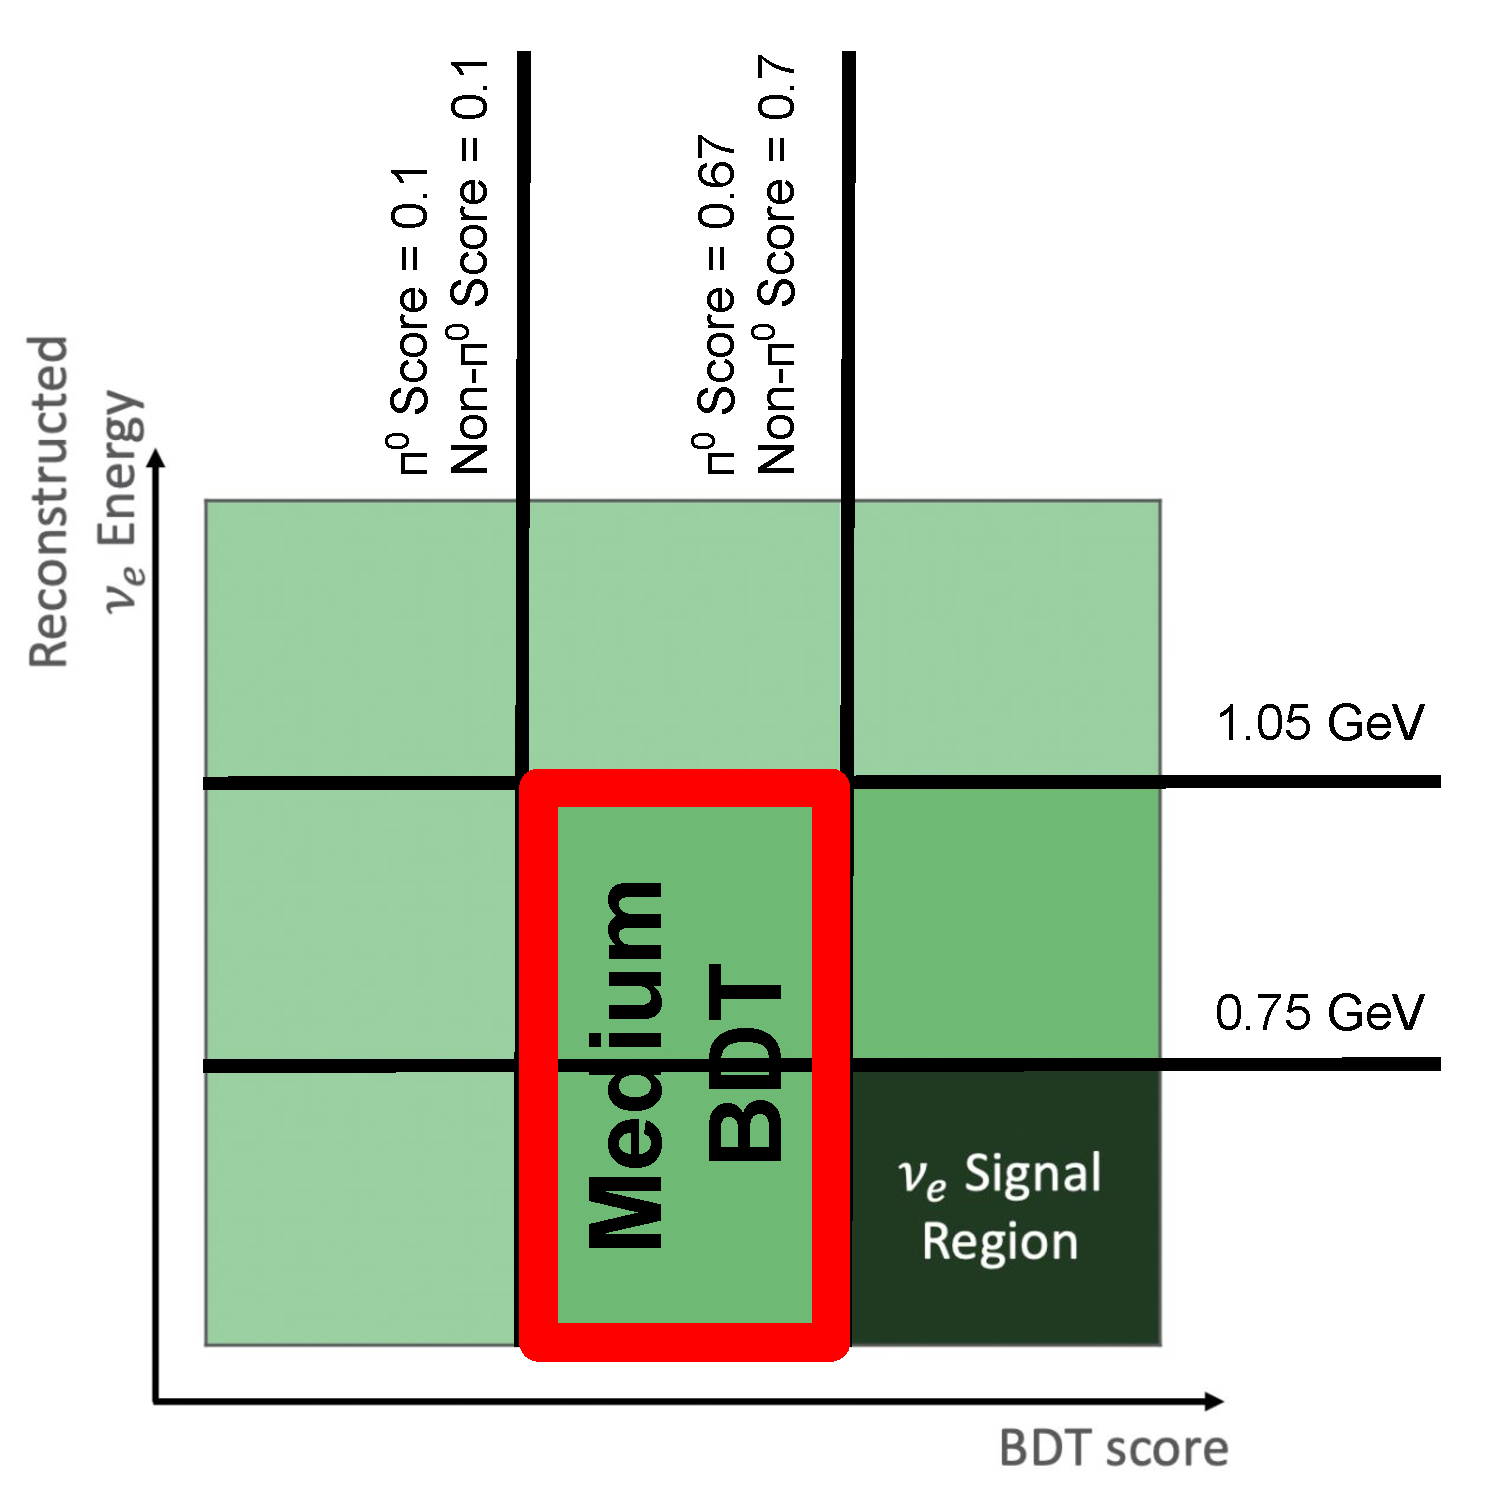
\includegraphics[width=\linewidth]{technote/Sidebands/Figures/NearSideband/NpMediumBDTSideband.pdf}
        \caption{For the 1eNp selection.}
    \end{subfigure}
    \caption{The BDT score sidebands.}
    \label{fig:MediumBDTSideband}
\end{figure}

\begin{figure}[H]
    \centering
    \begin{subfigure}{0.5\linewidth}
        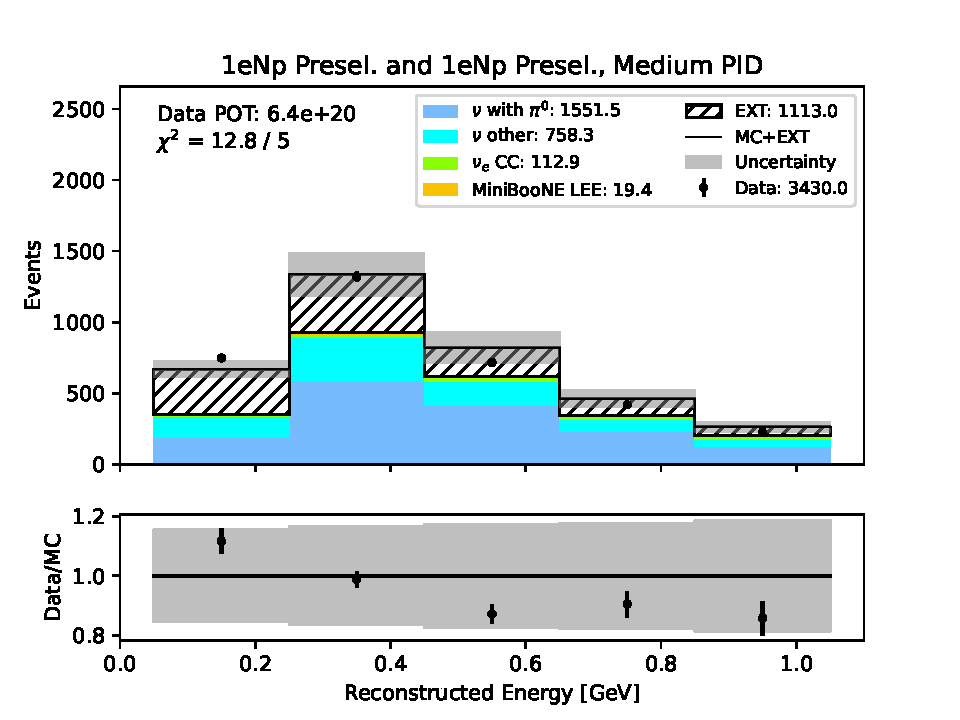
\includegraphics[width=\linewidth]{technote/Sidebands/Figures/NearSideband/near_sideband_reco_e_run123_NP_NP_MEDIUM_PID.pdf}
        \caption{$\nu_e$ preselection, runs 1-3.}
    \end{subfigure}%
    \begin{subfigure}{0.5\linewidth}
        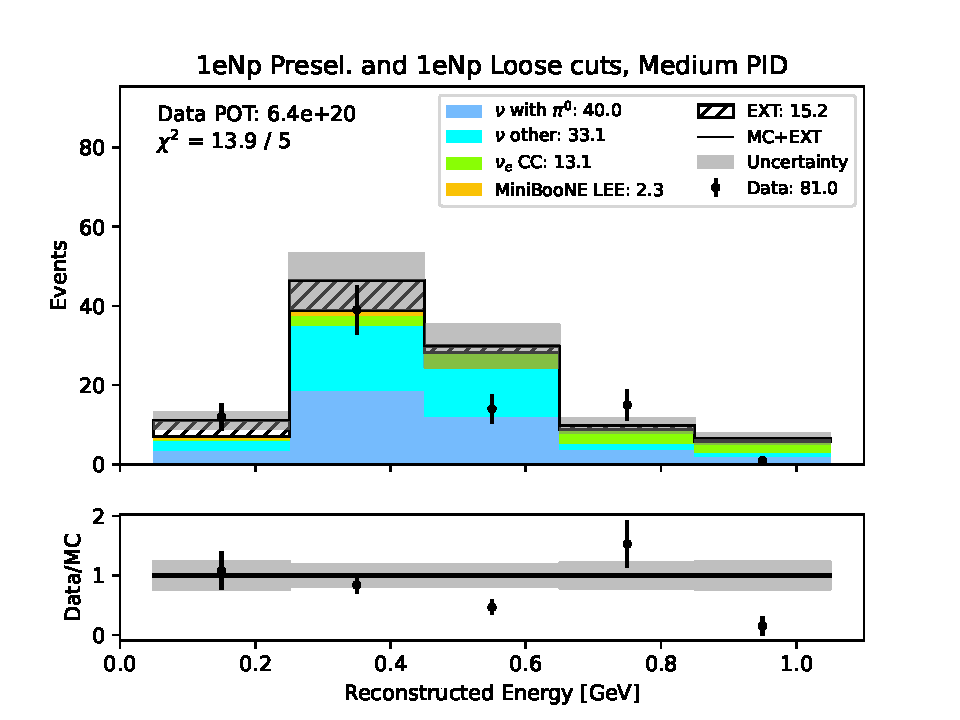
\includegraphics[width=\linewidth]{technote/Sidebands/Figures/NearSideband/near_sideband_reco_e_run123_NP_NPL_MEDIUM_PID.pdf}
        \caption{1eNp loose selection, runs 1-3.}
    \end{subfigure}
    \begin{subfigure}{0.5\linewidth}
        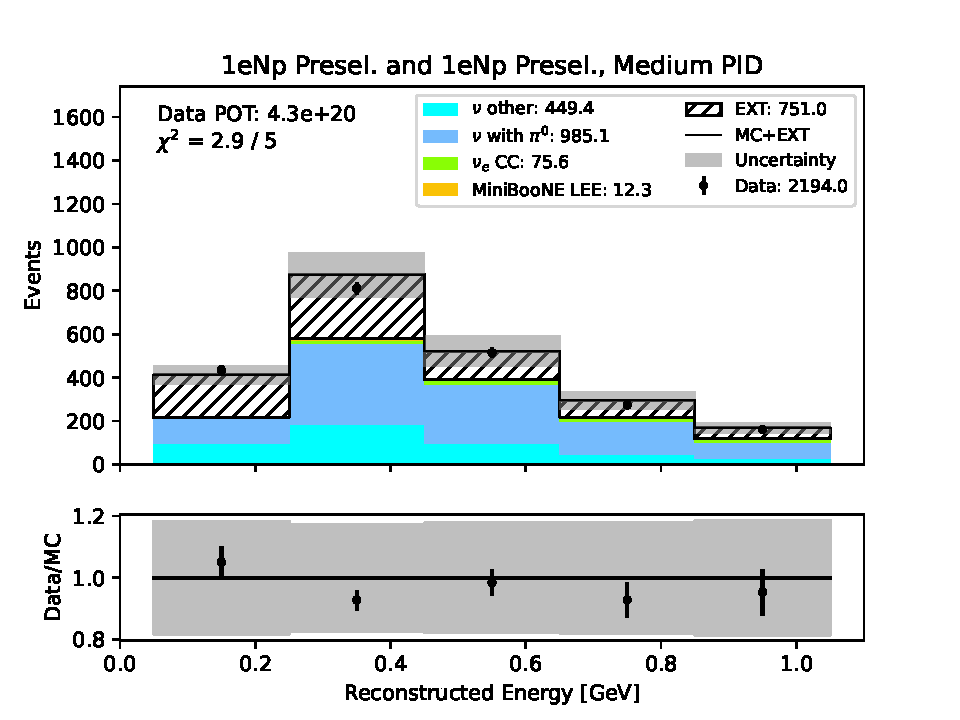
\includegraphics[width=\linewidth]{technote/Sidebands/Figures/NearSideband/near_sideband_reco_e_run4b4c4d5_NP_NP_MEDIUM_PID.pdf}
        \caption{$\nu_e$ preselection, runs 4-5.}
    \end{subfigure}%
    \begin{subfigure}{0.5\linewidth}
        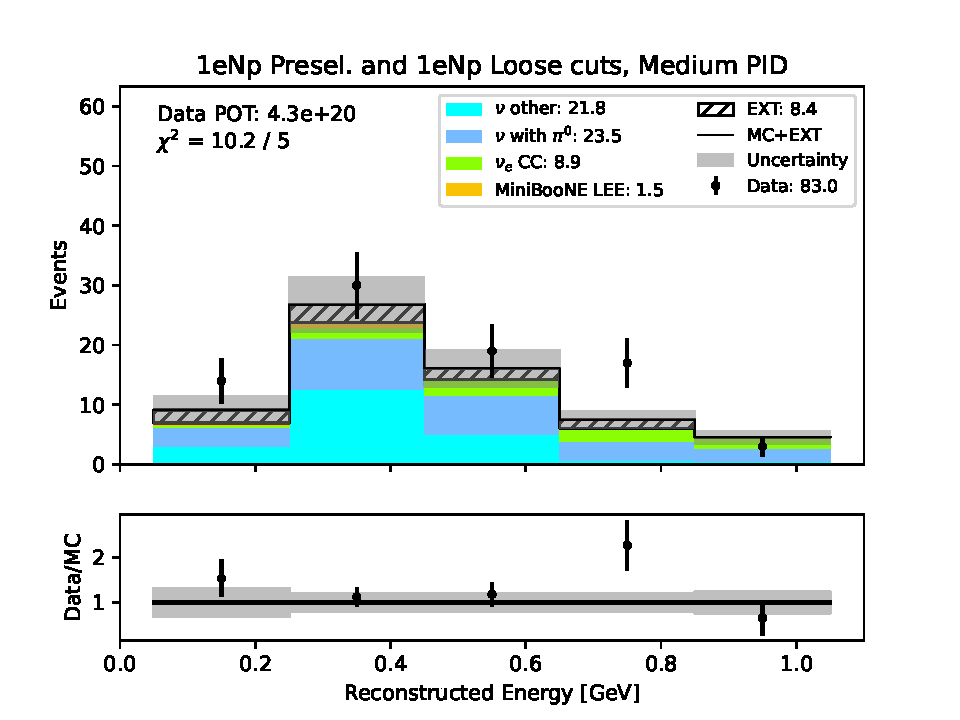
\includegraphics[width=\linewidth]{technote/Sidebands/Figures/NearSideband/near_sideband_reco_e_run4b4c4d5_NP_NPL_MEDIUM_PID.pdf}
        \caption{1eNp loose selection, runs 4-5.}
    \end{subfigure}    
    \begin{subfigure}{0.5\linewidth}
        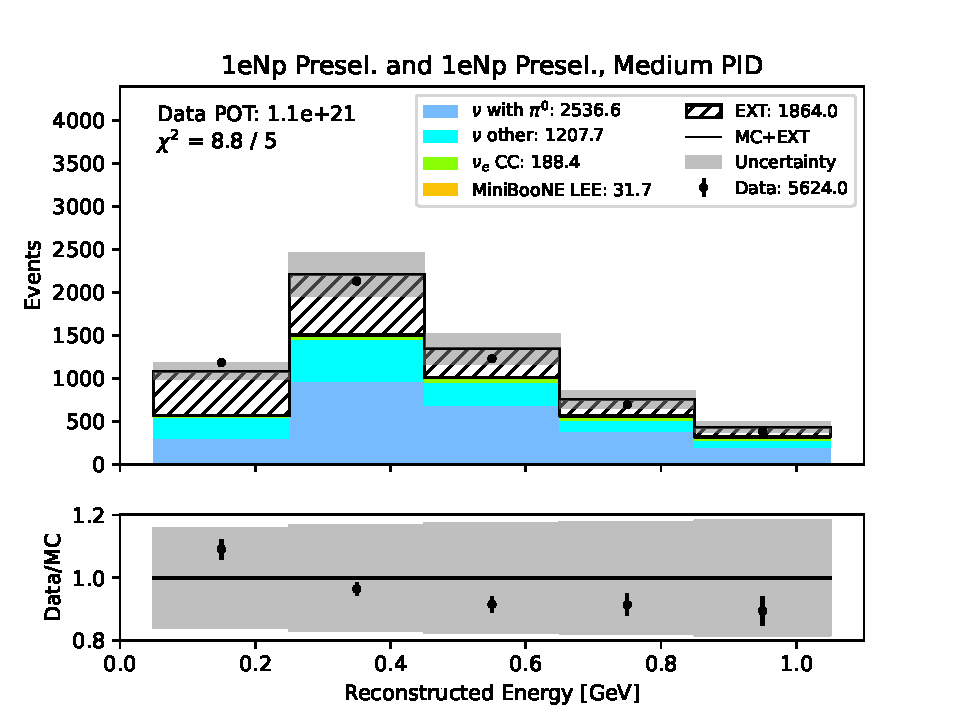
\includegraphics[width=\linewidth]{technote/Sidebands/Figures/NearSideband/near_sideband_reco_e_run1234b4c4d5_NP_NP_MEDIUM_PID.pdf}
        \caption{$\nu_e$ preselection, runs 1-5.}
    \end{subfigure}%
    \begin{subfigure}{0.5\linewidth}
        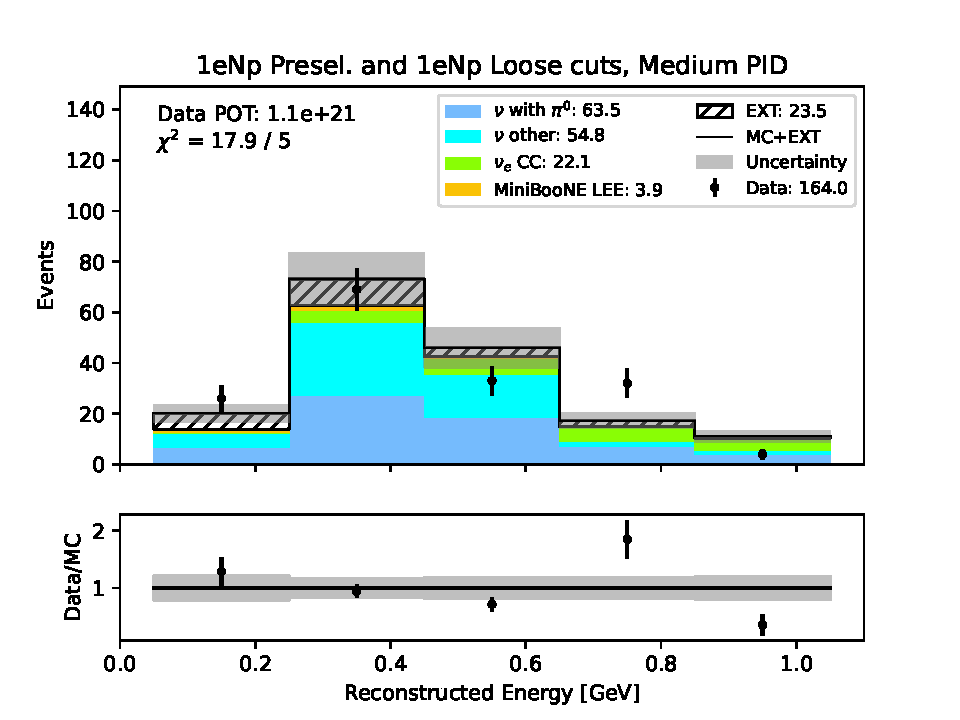
\includegraphics[width=\linewidth]{technote/Sidebands/Figures/NearSideband/near_sideband_reco_e_run1234b4c4d5_NP_NPL_MEDIUM_PID.pdf}
        \caption{1eNp loose selection, runs 1-5.}
    \end{subfigure}
    \caption{Data and MC simulation comparisons in the 1eNp medium BDT score sideband.}
\end{figure}

\begin{figure}[H]
    \centering
    \begin{subfigure}{0.5\linewidth}
        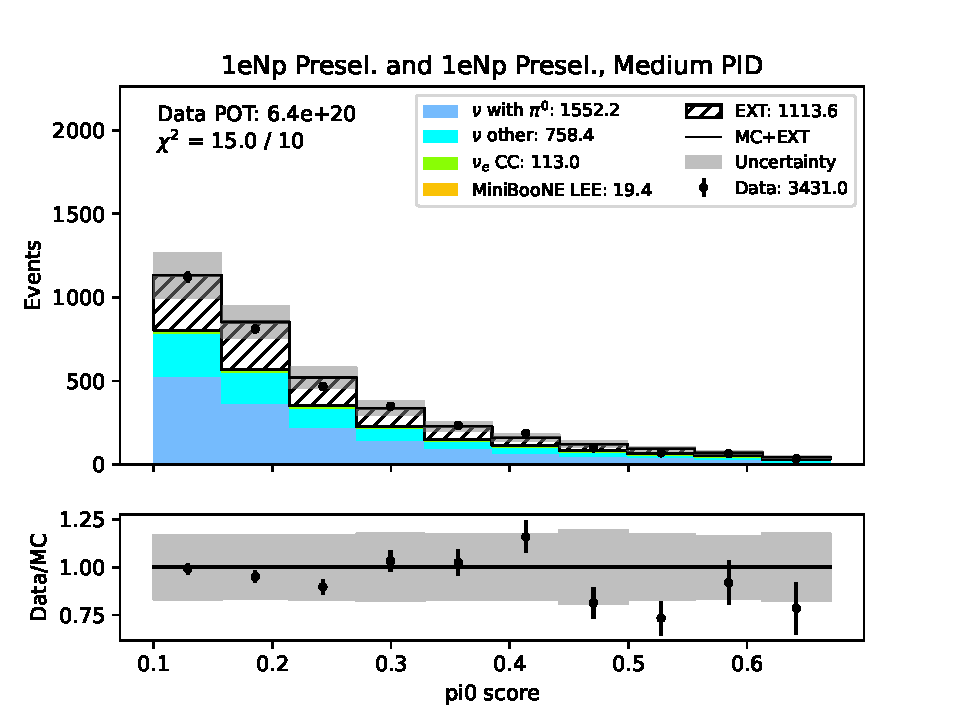
\includegraphics[width=\linewidth]{technote/Sidebands/Figures/NearSideband/near_sideband_pi0_score_run123_NP_NP_MEDIUM_PID.pdf}
        \caption{$\nu_e$ preselection, runs 1-3.}
    \end{subfigure}%
    \begin{subfigure}{0.5\linewidth}
        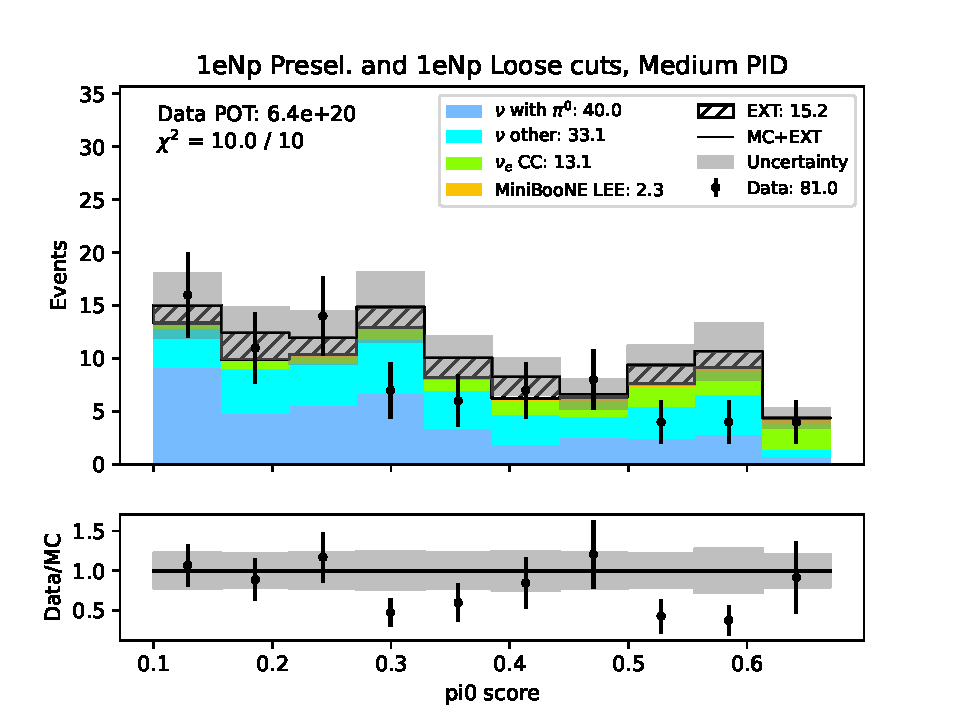
\includegraphics[width=\linewidth]{technote/Sidebands/Figures/NearSideband/near_sideband_pi0_score_run123_NP_NPL_MEDIUM_PID.pdf}
        \caption{1eNp loose selection, runs 1-3.}
    \end{subfigure}
    \begin{subfigure}{0.5\linewidth}
        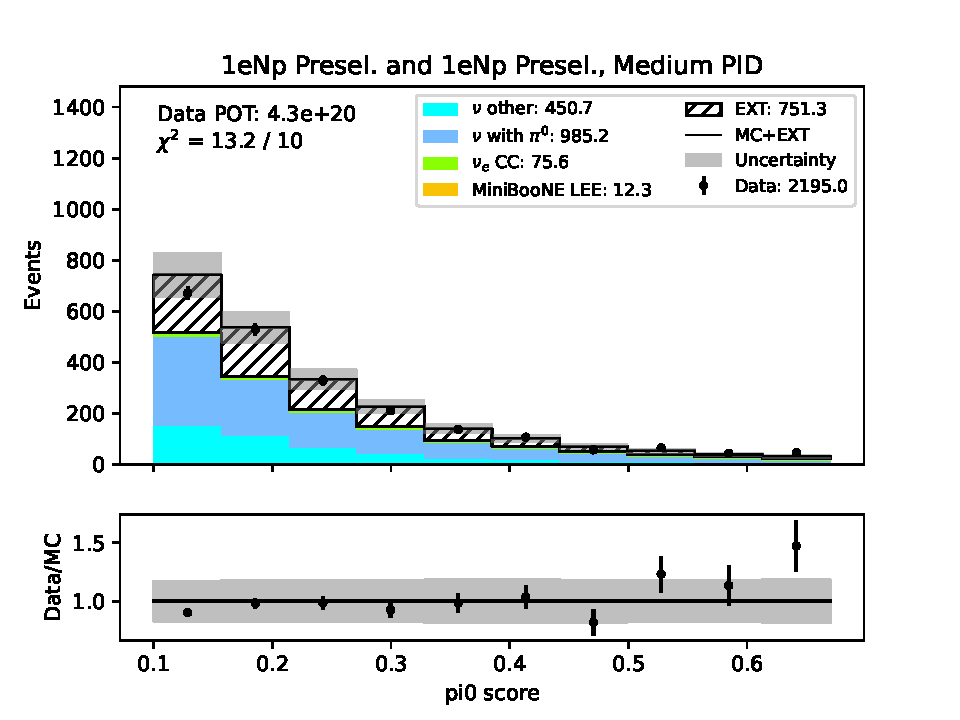
\includegraphics[width=\linewidth]{technote/Sidebands/Figures/NearSideband/near_sideband_pi0_score_run4b4c4d5_NP_NP_MEDIUM_PID.pdf}
        \caption{$\nu_e$ preselection, runs 4-5.}
    \end{subfigure}%
    \begin{subfigure}{0.5\linewidth}
        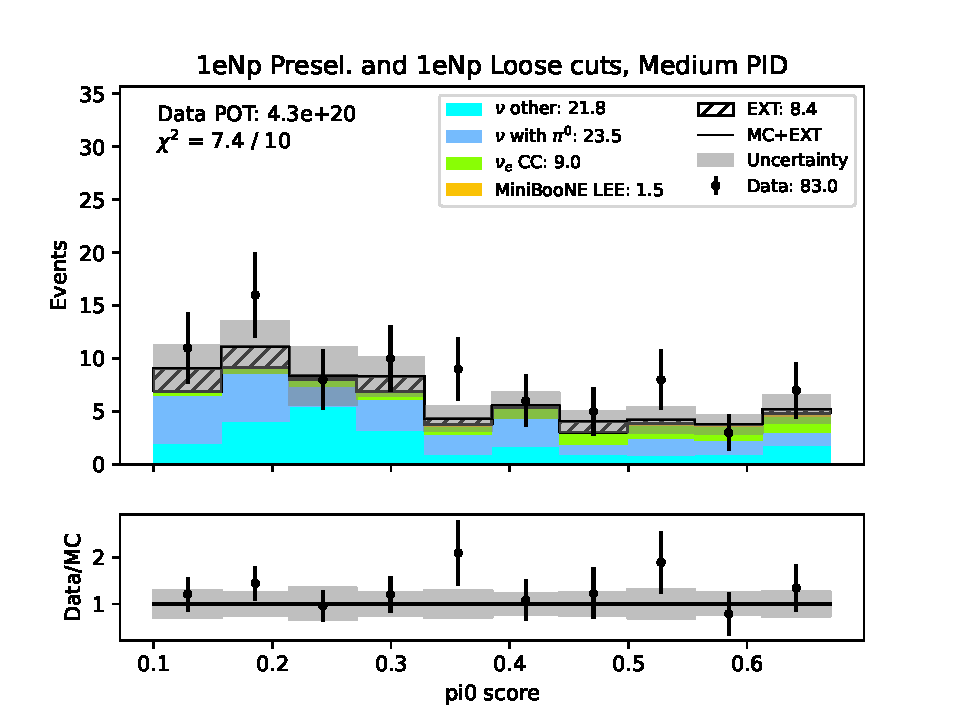
\includegraphics[width=\linewidth]{technote/Sidebands/Figures/NearSideband/near_sideband_pi0_score_run4b4c4d5_NP_NPL_MEDIUM_PID.pdf}
        \caption{1eNp loose selection, runs 4-5.}
    \end{subfigure}    
    \begin{subfigure}{0.5\linewidth}
        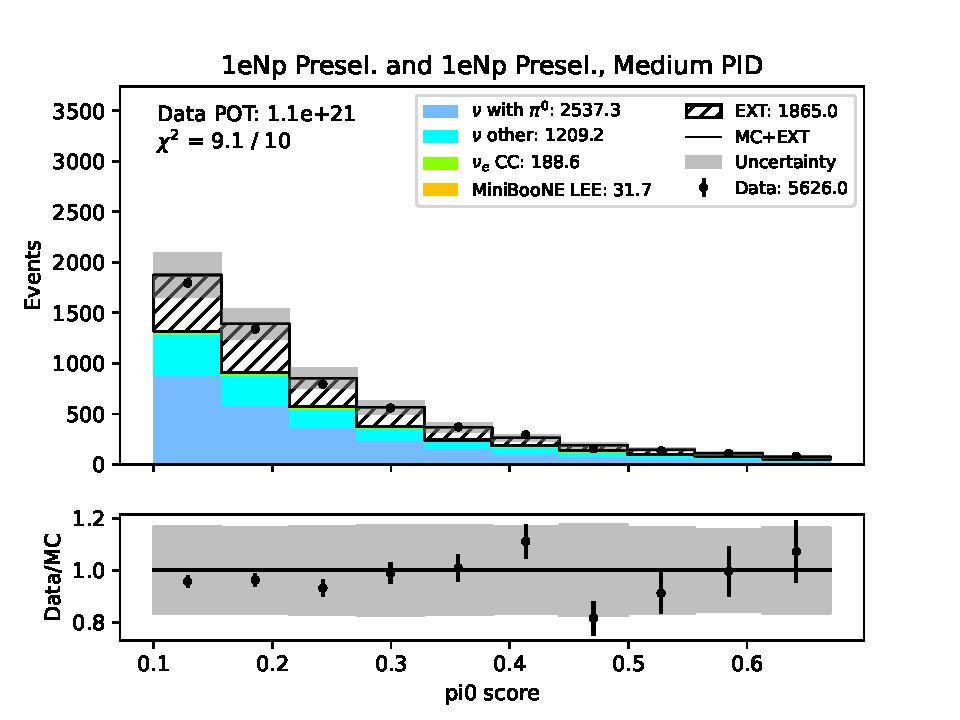
\includegraphics[width=\linewidth]{technote/Sidebands/Figures/NearSideband/near_sideband_pi0_score_run1234b4c4d5_NP_NP_MEDIUM_PID.pdf}
        \caption{$\nu_e$ preselection, runs 1-5.}
    \end{subfigure}%
    \begin{subfigure}{0.5\linewidth}
        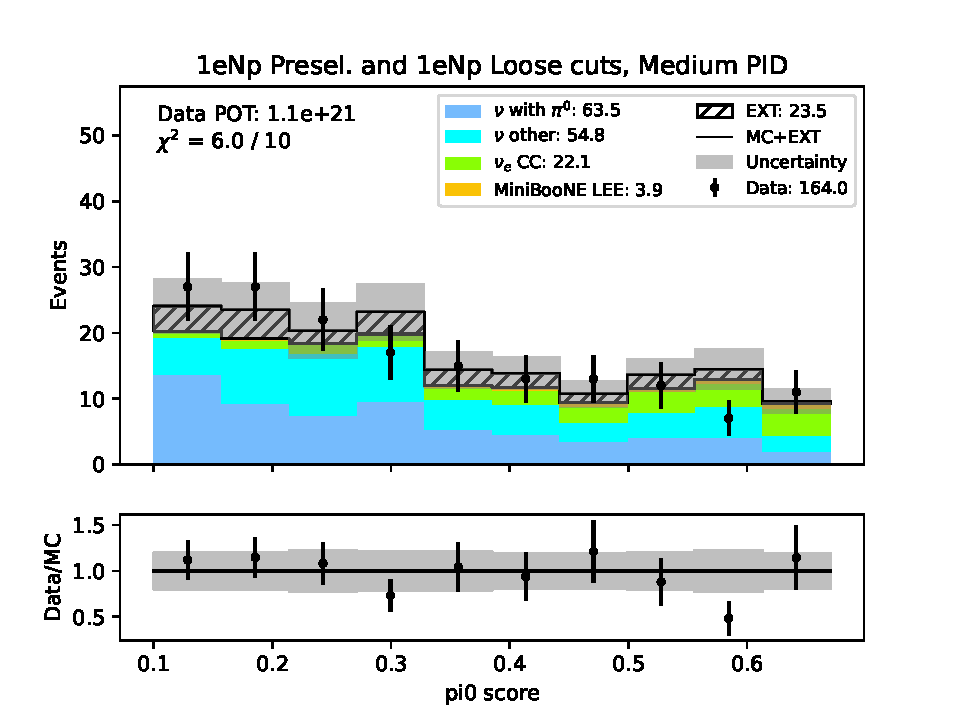
\includegraphics[width=\linewidth]{technote/Sidebands/Figures/NearSideband/near_sideband_pi0_score_run1234b4c4d5_NP_NPL_MEDIUM_PID.pdf}
        \caption{1eNp loose selection, runs 1-5.}
    \end{subfigure}
    \caption{Data and MC simulation comparisons in the 1eNp medium BDT score sideband.}
\end{figure}

\begin{figure}[H]
    \centering
    \begin{subfigure}{0.5\linewidth}
        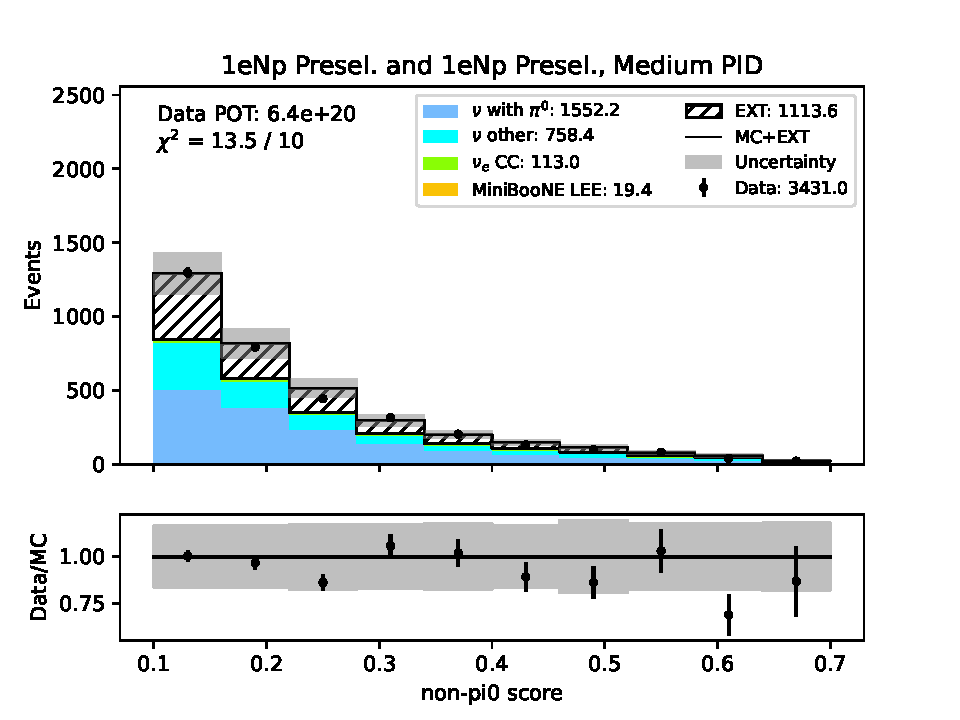
\includegraphics[width=\linewidth]{technote/Sidebands/Figures/NearSideband/near_sideband_nonpi0_score_run123_NP_NP_MEDIUM_PID.pdf}
        \caption{$\nu_e$ preselection, runs 1-3.}
    \end{subfigure}%
    \begin{subfigure}{0.5\linewidth}
        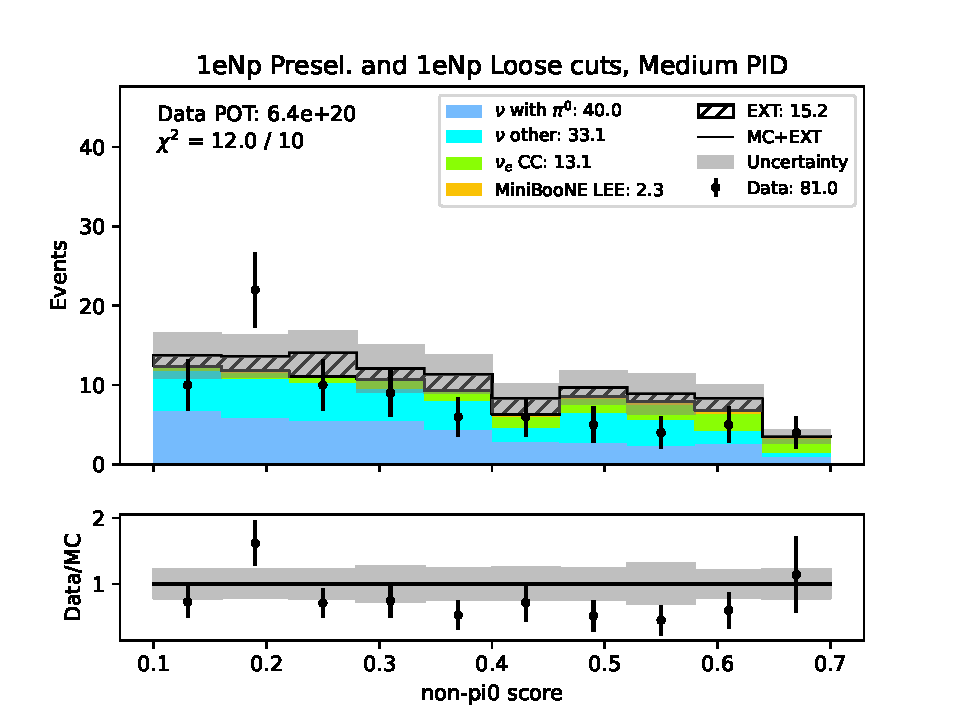
\includegraphics[width=\linewidth]{technote/Sidebands/Figures/NearSideband/near_sideband_nonpi0_score_run123_NP_NPL_MEDIUM_PID.pdf}
        \caption{1eNp loose selection, runs 1-3.}
    \end{subfigure}
    \begin{subfigure}{0.5\linewidth}
        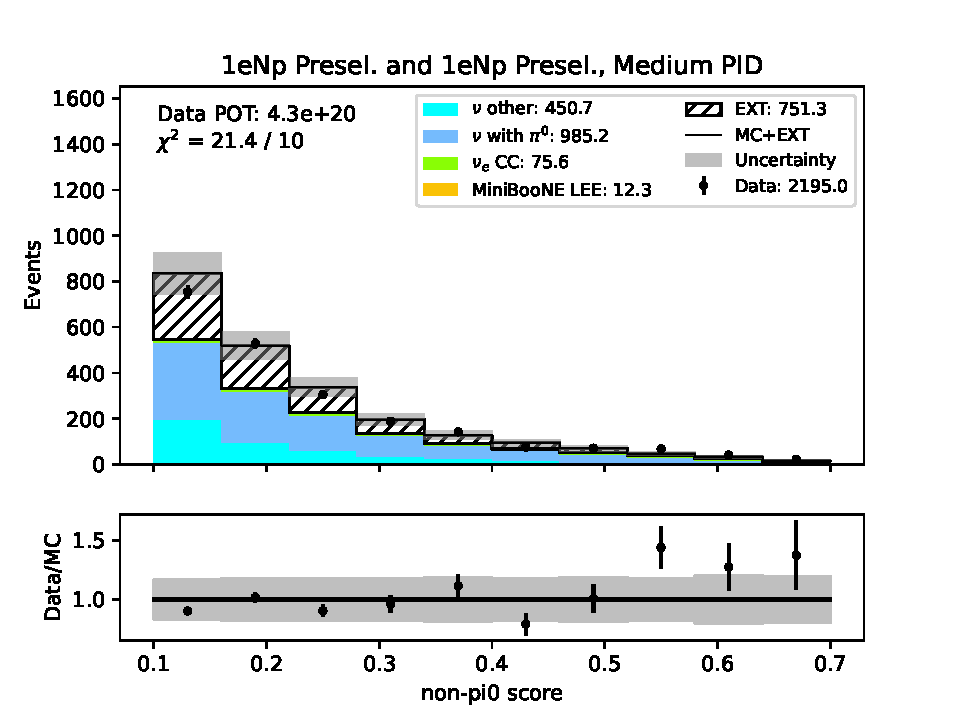
\includegraphics[width=\linewidth]{technote/Sidebands/Figures/NearSideband/near_sideband_nonpi0_score_run4b4c4d5_NP_NP_MEDIUM_PID.pdf}
        \caption{$\nu_e$ preselection, runs 4-5.}
    \end{subfigure}%
    \begin{subfigure}{0.5\linewidth}
        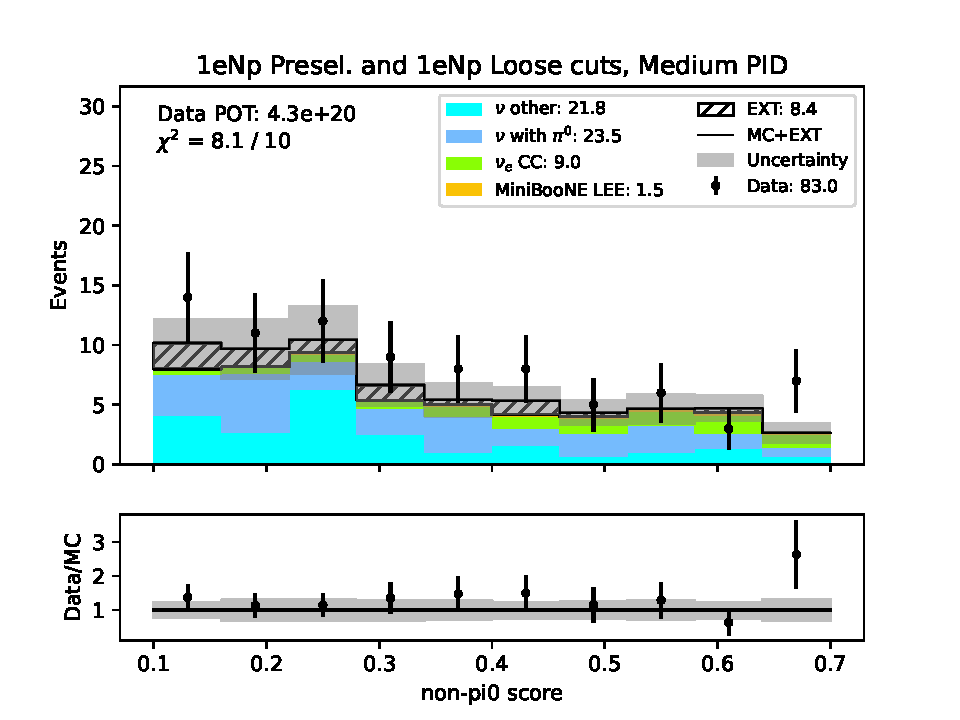
\includegraphics[width=\linewidth]{technote/Sidebands/Figures/NearSideband/near_sideband_nonpi0_score_run4b4c4d5_NP_NPL_MEDIUM_PID.pdf}
        \caption{1eNp loose selection, runs 4-5.}
    \end{subfigure}    
    \begin{subfigure}{0.5\linewidth}
        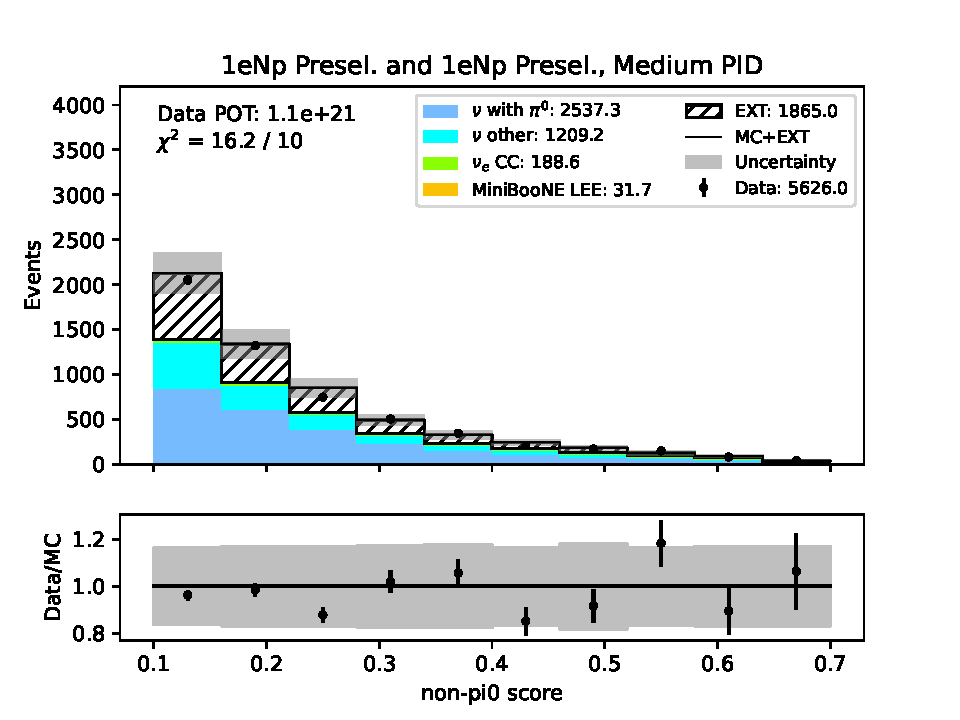
\includegraphics[width=\linewidth]{technote/Sidebands/Figures/NearSideband/near_sideband_nonpi0_score_run1234b4c4d5_NP_NP_MEDIUM_PID.pdf}
        \caption{$\nu_e$ preselection, runs 1-5.}
    \end{subfigure}%
    \begin{subfigure}{0.5\linewidth}
        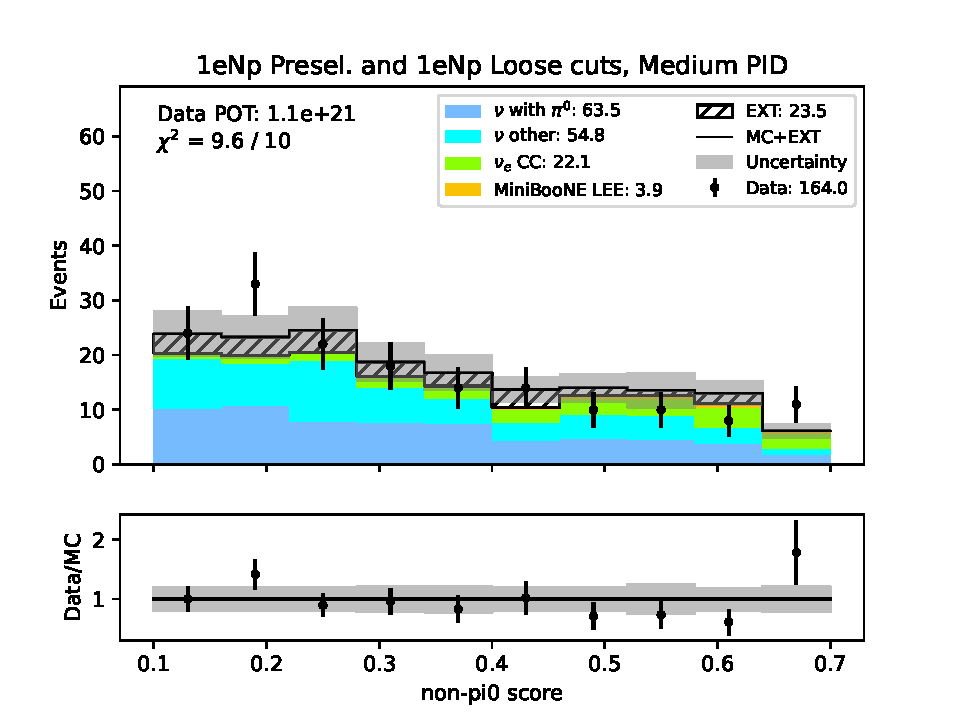
\includegraphics[width=\linewidth]{technote/Sidebands/Figures/NearSideband/near_sideband_nonpi0_score_run1234b4c4d5_NP_NPL_MEDIUM_PID.pdf}
        \caption{1eNp loose selection, runs 1-5.}
    \end{subfigure}
    \caption{Data and MC simulation comparisons in the 1e0p medium BDT score sideband.}
\end{figure}

\begin{figure}[H]
    \centering
    \begin{subfigure}{0.5\linewidth}
        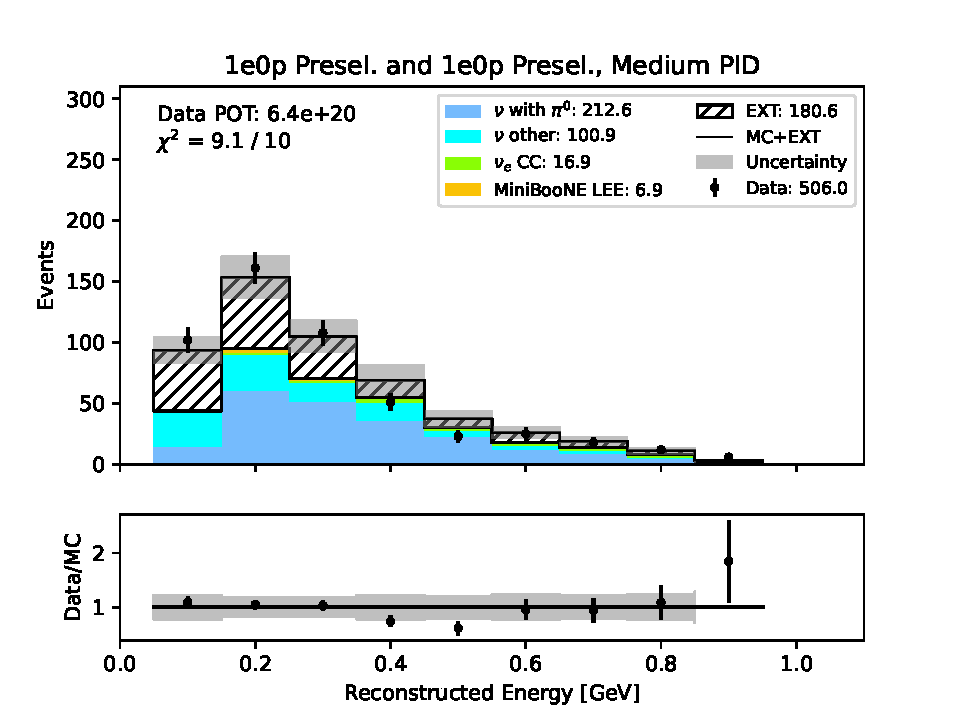
\includegraphics[width=\linewidth]{technote/Sidebands/Figures/NearSideband/near_sideband_reco_e_run123_ZP_ZP_MEDIUM_PID.pdf}
        \caption{$\nu_e$ preselection, runs 1-3.}
    \end{subfigure}%
    \begin{subfigure}{0.5\linewidth}
        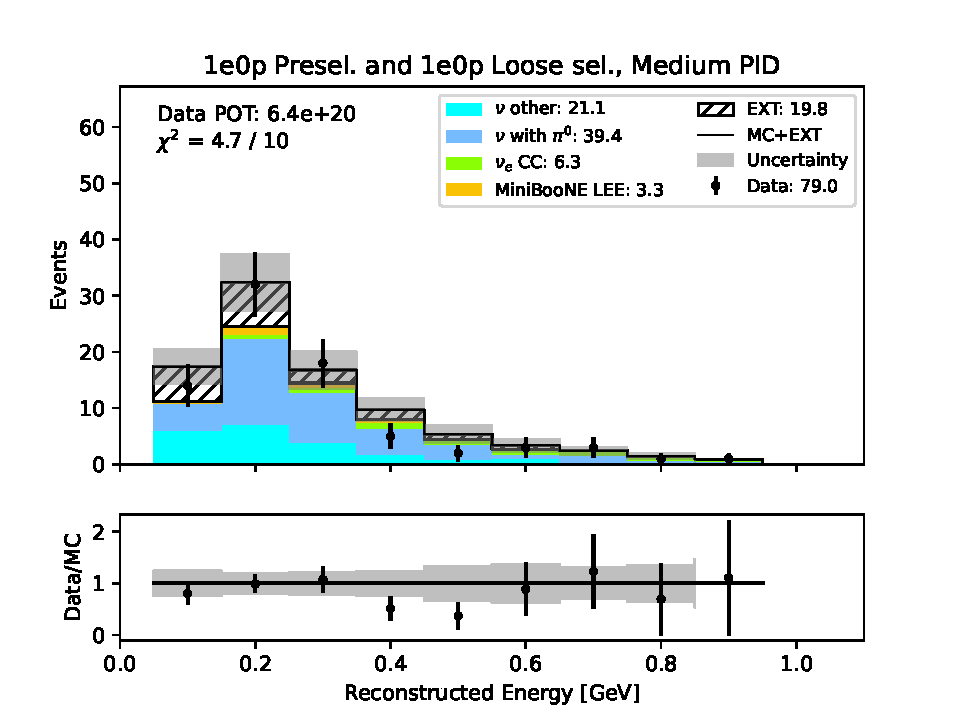
\includegraphics[width=\linewidth]{technote/Sidebands/Figures/NearSideband/near_sideband_reco_e_run123_ZP_ZPLOOSESEL_MEDIUM_PID.pdf}
        \caption{1e0p loose selection, runs 1-3.}
    \end{subfigure}
    \begin{subfigure}{0.5\linewidth}
        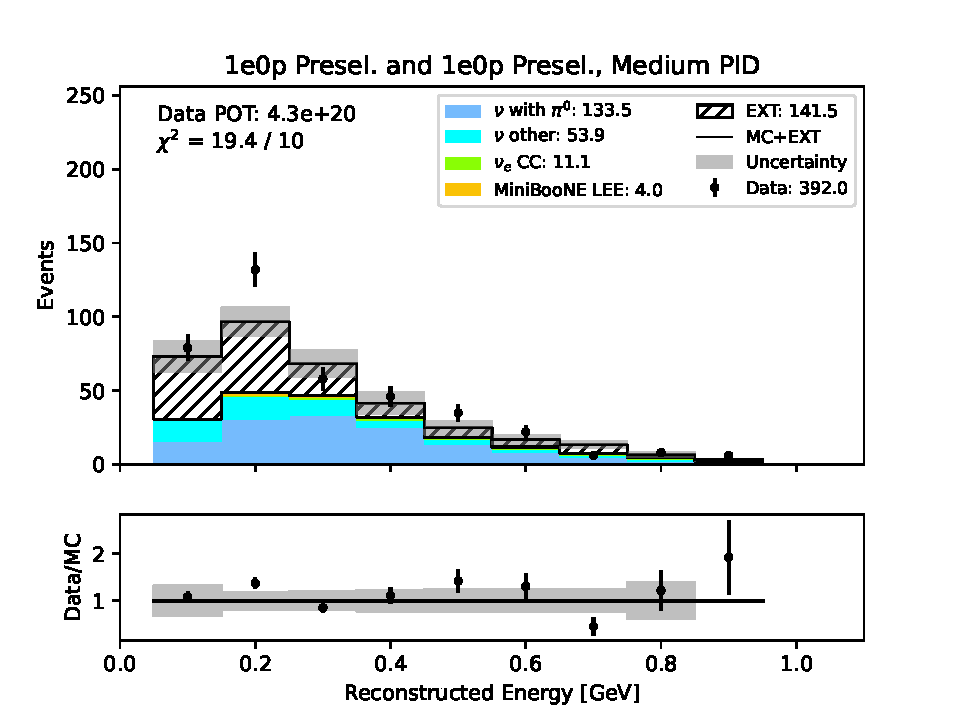
\includegraphics[width=\linewidth]{technote/Sidebands/Figures/NearSideband/near_sideband_reco_e_run4b4c4d5_ZP_ZP_MEDIUM_PID.pdf}
        \caption{$\nu_e$ preselection, runs 4-5.}
    \end{subfigure}%
    \begin{subfigure}{0.5\linewidth}
        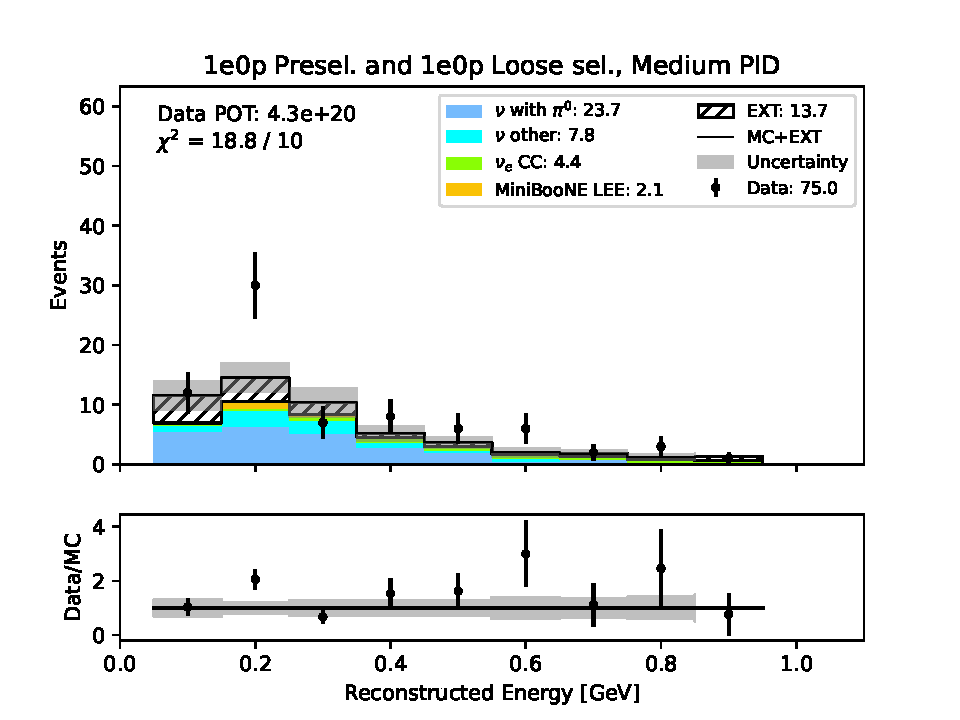
\includegraphics[width=\linewidth]{technote/Sidebands/Figures/NearSideband/near_sideband_reco_e_run4b4c4d5_ZP_ZPLOOSESEL_MEDIUM_PID.pdf}
        \caption{1e0p loose selection, runs 4-5.}
    \end{subfigure}    
    \begin{subfigure}{0.5\linewidth}
        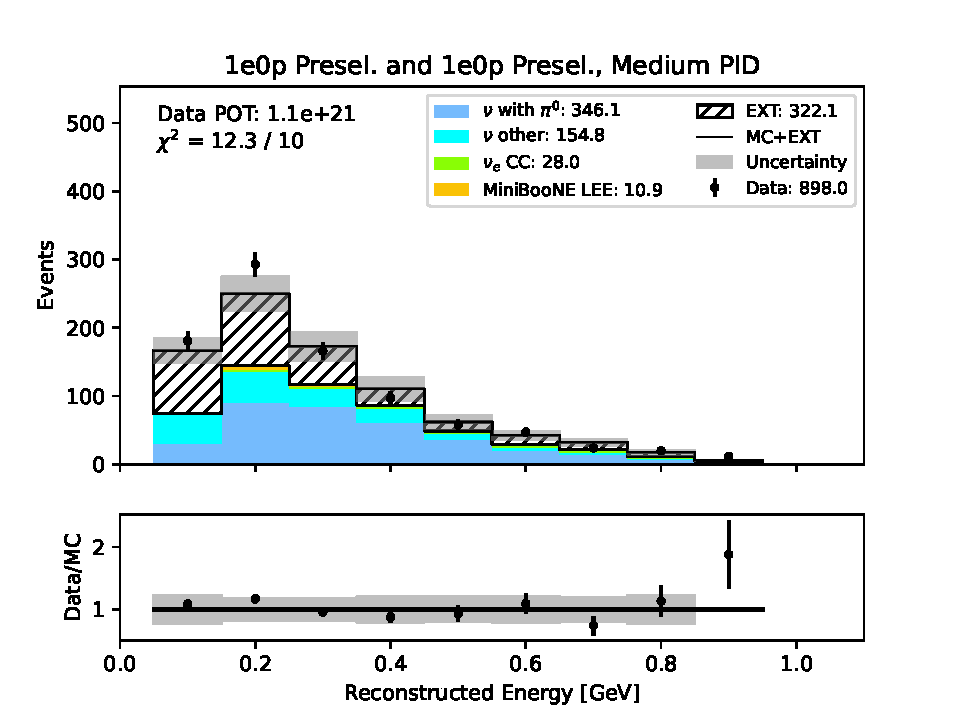
\includegraphics[width=\linewidth]{technote/Sidebands/Figures/NearSideband/near_sideband_reco_e_run1234b4c4d5_ZP_ZP_MEDIUM_PID.pdf}
        \caption{$\nu_e$ preselection, runs 1-5.}
    \end{subfigure}%
    \begin{subfigure}{0.5\linewidth}
        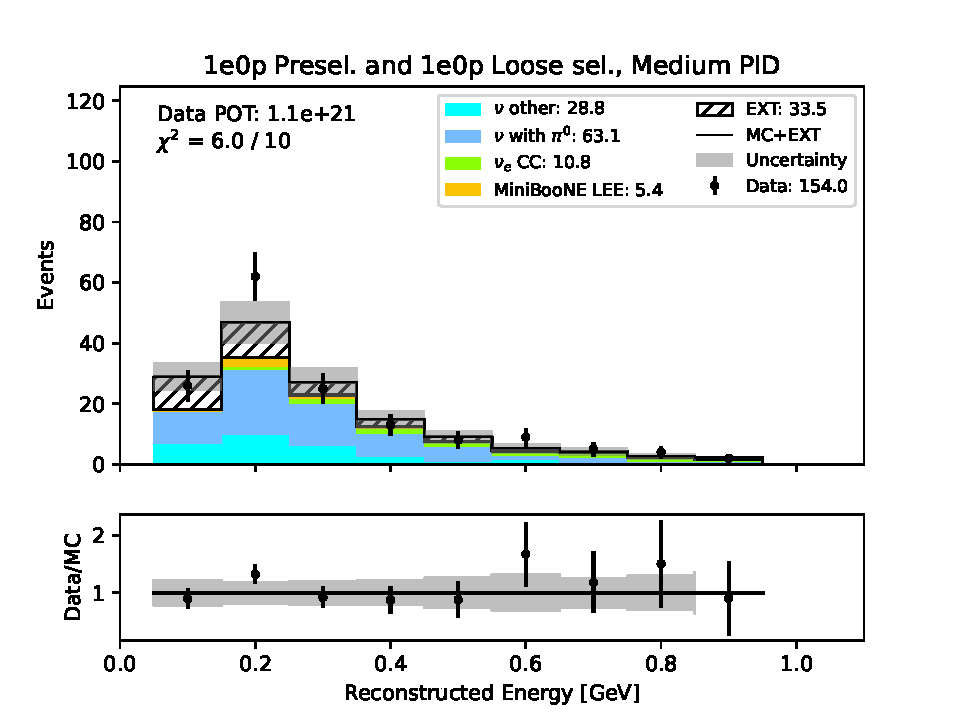
\includegraphics[width=\linewidth]{technote/Sidebands/Figures/NearSideband/near_sideband_reco_e_run1234b4c4d5_ZP_ZPLOOSESEL_MEDIUM_PID.pdf}
        \caption{1e0p loose selection, runs 1-5.}
    \end{subfigure}
    \caption{Data and MC simulation comparisons in the 1e0p medium BDT score sideband.}
\end{figure}

\begin{figure}[H]
    \centering
    \begin{subfigure}{0.5\linewidth}
        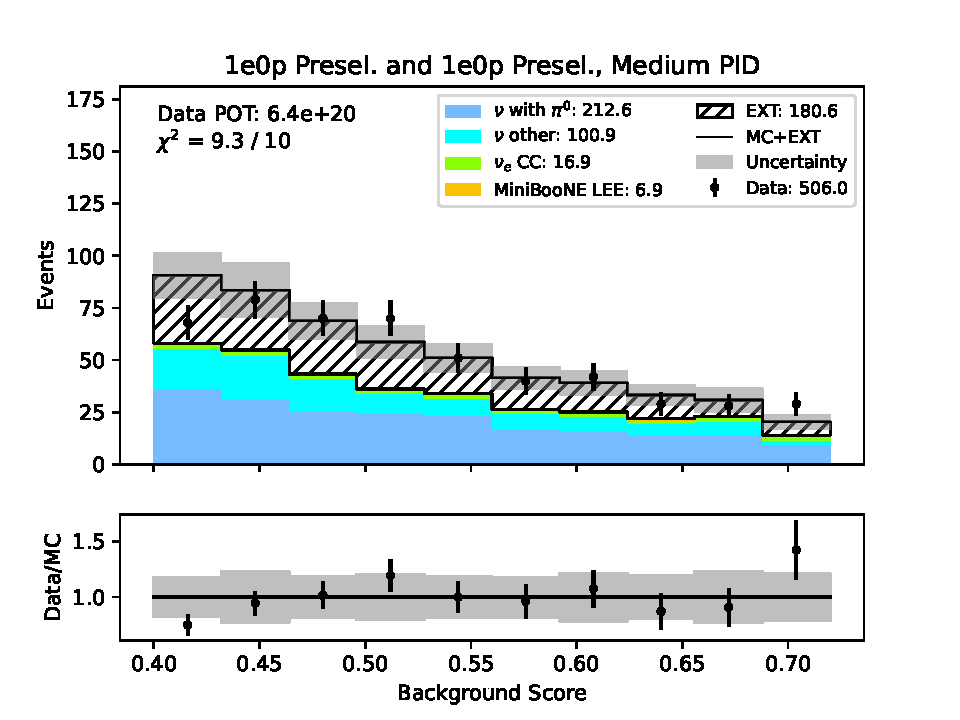
\includegraphics[width=\linewidth]{technote/Sidebands/Figures/NearSideband/near_sideband_bkg_score_run123_ZP_ZP_MEDIUM_PID.pdf}
        \caption{$\nu_e$ preselection, runs 1-3.}
    \end{subfigure}%
    \begin{subfigure}{0.5\linewidth}
        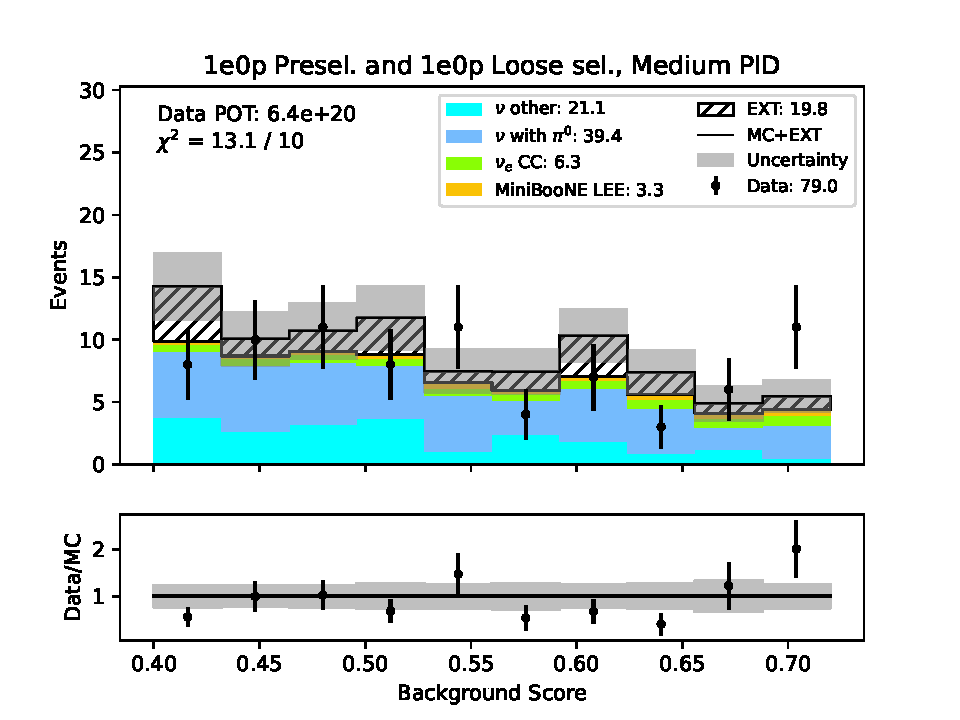
\includegraphics[width=\linewidth]{technote/Sidebands/Figures/NearSideband/near_sideband_bkg_score_run123_ZP_ZPLOOSESEL_MEDIUM_PID.pdf}
        \caption{1e0p loose selection, runs 1-3.}
    \end{subfigure}
    \begin{subfigure}{0.5\linewidth}
        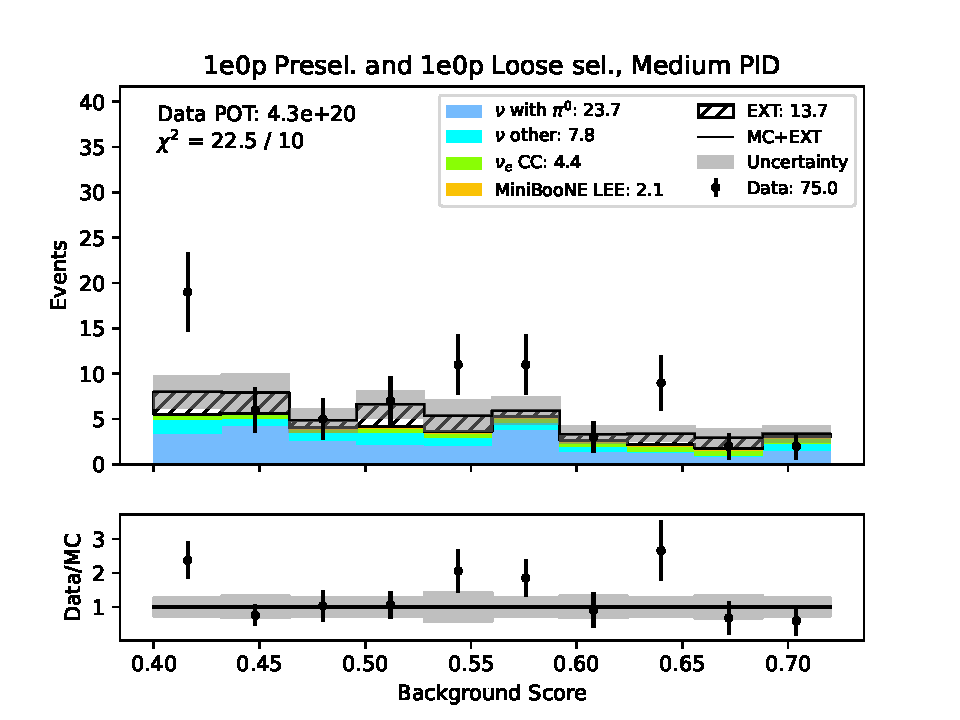
\includegraphics[width=\linewidth]{technote/Sidebands/Figures/NearSideband/near_sideband_bkg_score_run4b4c4d5_ZP_ZPLOOSESEL_MEDIUM_PID.pdf}
        \caption{$\nu_e$ preselection, runs 4-5.}
    \end{subfigure}%
    \begin{subfigure}{0.5\linewidth}
        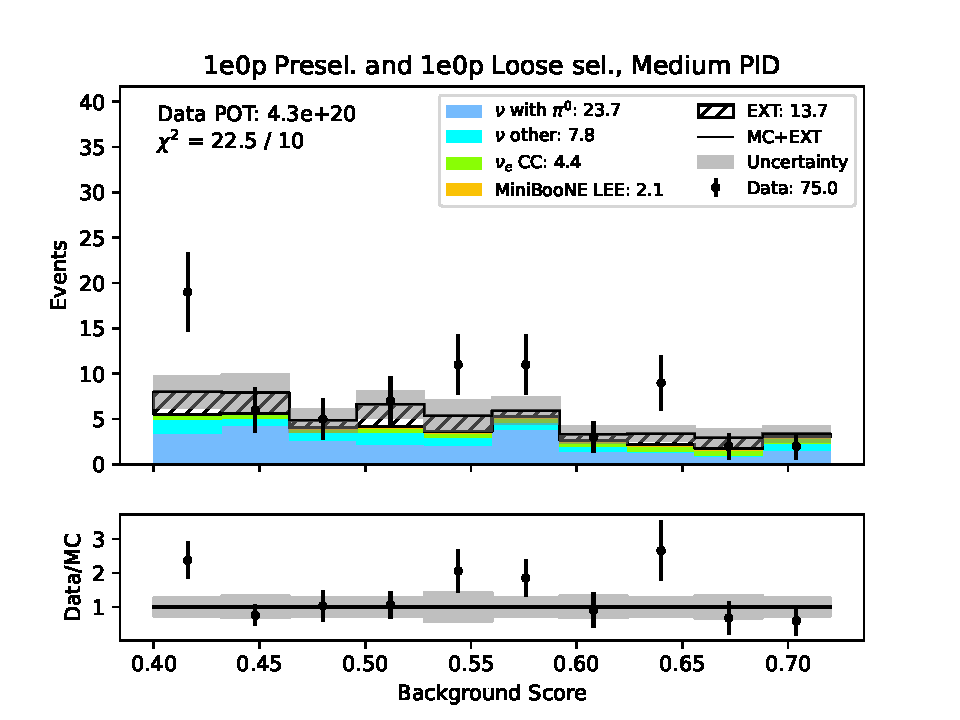
\includegraphics[width=\linewidth]{technote/Sidebands/Figures/NearSideband/near_sideband_bkg_score_run4b4c4d5_ZP_ZPLOOSESEL_MEDIUM_PID.pdf}
        \caption{1e0p loose selection, runs 4-5.}
    \end{subfigure}    
    \begin{subfigure}{0.5\linewidth}
        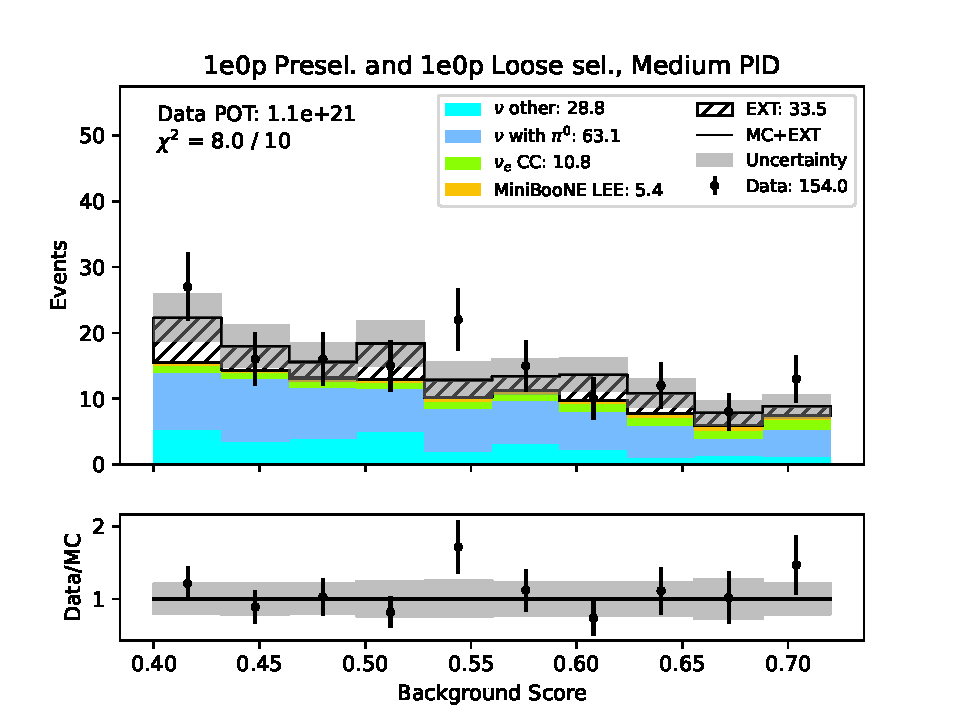
\includegraphics[width=\linewidth]{technote/Sidebands/Figures/NearSideband/near_sideband_bkg_score_run1234b4c4d5_ZP_ZPLOOSESEL_MEDIUM_PID.pdf}
        \caption{$\nu_e$ preselection, runs 1-5.}
    \end{subfigure}%
    \begin{subfigure}{0.5\linewidth}
        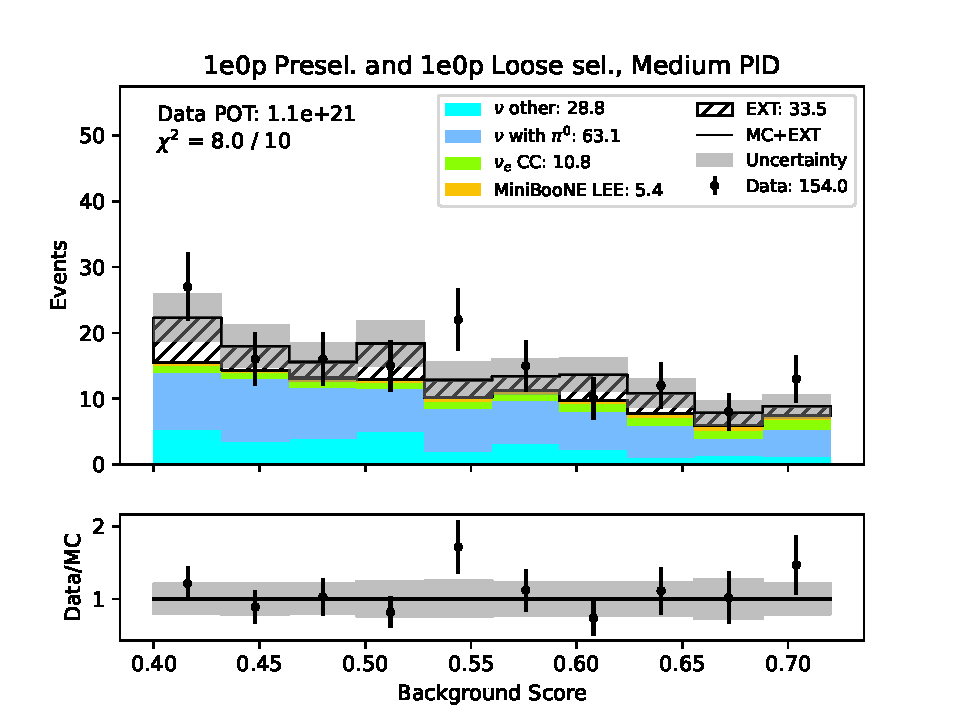
\includegraphics[width=\linewidth]{technote/Sidebands/Figures/NearSideband/near_sideband_bkg_score_run1234b4c4d5_ZP_ZPLOOSESEL_MEDIUM_PID.pdf}
        \caption{1e0p loose selection, runs 1-5.}
    \end{subfigure}
    \caption{Data and MC simulation comparisons in the 1e0p medium BDT score sideband.}
\end{figure}